\documentclass[aspectratio=169,11pt]{beamer}

\usetheme{metropolis}
\usepackage{booktabs}
\usepackage{graphicx}
\usepackage{tikz}
\usepackage{xcolor}
\usepackage{array}
\usetikzlibrary{arrows.meta,positioning,shapes.geometric,fit,calc}

\definecolor{accent}{HTML}{0077B6}
\definecolor{muted}{HTML}{6C757D}
\definecolor{gold}{HTML}{FBBF24}
\definecolor{good}{HTML}{10B981}
\definecolor{bad}{HTML}{EF4444}
\definecolor{mid}{HTML}{FBBF24}
\setbeamercolor{frametitle}{bg=accent,fg=white}
\setbeamercolor{progress bar}{fg=accent}
\setbeamercolor{alerted text}{fg=accent}

\title{Data Lakehouse --- Biweekly Progress}
\subtitle{Nvidia PhysicalAI Ingestion \& Cosmos Augmentation}
\date{April 2026}
\author{}
\institute{NetAI Digital Twin Project}

\begin{document}

\maketitle

% ==========================================================================
% SLIDE 1
% ==========================================================================
\begin{frame}{Nvidia PhysicalAI AV Dataset --- Ingestion \& Overhead Reduction
  \hfill\colorbox{good!20}{\scriptsize\textcolor{good}{\textbf{COMPLETE}}}}

\begin{columns}[T]

\begin{column}{0.56\textwidth}

{\footnotesize\textbf{\textcolor{accent}{PART 1 --- PIPELINE VALIDATED AT SCALE}}}\\[3pt]
{\scriptsize
Full Bronze $\to$ Silver $\to$ Gold medallion pipeline for
the Nvidia PhysicalAI AV dataset (310,895 clips, 14 sensor types, 41 tables/tier).
Benchmarked 2--75 clips: linear scaling (R$^2 > 0.99$) at constant marginal cost per clip.
}

\vspace{3pt}
{\scriptsize
\begin{tabular}{@{}lrl@{}}
\toprule
Metric & Per-clip cost & R\textsuperscript{2} \\
\midrule
Peak memory & \textbf{\textcolor{gold}{421\,MB}}/clip + 944\,MB base & 0.995 \\
Wall time & \textbf{\textcolor{gold}{53.9\,s}}/clip + 117\,s base & 0.993 \\
Rows ingested & \textbf{\textcolor{gold}{4.74\,M}}/clip + 9.3\,M base & 0.989 \\
\bottomrule
\end{tabular}
}

\vspace{6pt}
{\footnotesize\textbf{\textcolor{accent}{PART 2 --- STORAGE OVERHEAD REDUCTION}}}\\[2pt]
{\tiny\color{muted} Naive all-materialized medallion tiers replicate data at each layer.
Three strategies benchmarked to reduce overhead while preserving tier guarantees:}

\vspace{3pt}
{\scriptsize
\begin{tabular}{@{}p{2.7cm}cccr@{}}
\toprule
Strategy & Silver & Gold & Total & Projected \\
\midrule
\textcolor{bad}{All materialized} & +100\% & +30\% & \textbf{\textcolor{gold}{2.3$\times$}} & 388\,TB \\
\textcolor{mid}{View Silver + mat.\ Gold} & +0\% & +30\% & \textbf{\textcolor{gold}{1.3$\times$}} & 220\,TB \\
\rowcolor{good!8}
\textcolor{good}{View Silver + view Gold} & +0\% & +0\% & \textbf{\textcolor{gold}{1.0$\times$}} & 169\,TB \\
\bottomrule
\end{tabular}
}

\vspace{3pt}
{\tiny\color{muted}
All three strategies produce identical query interfaces. Gold views use
\texttt{CACHE TABLE} for hot-path queries (in-memory, ephemeral).
Switchable at runtime via \texttt{-{}-gold-mode} flag.
Source data: 169\,TB (311K clips $\times$ 555\,MB/clip).}

\end{column}

\begin{column}{0.42\textwidth}

{\footnotesize\textbf{\textcolor{accent}{ARCHITECTURE}}}

\vspace{2pt}
\centering
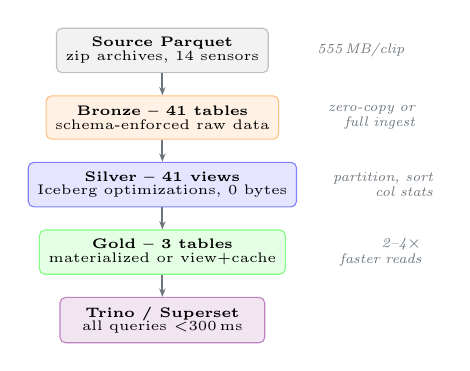
\begin{tikzpicture}[
    node distance=0.35cm,
    every node/.style={font=\tiny, align=center},
    box/.style={draw, rounded corners=2pt, minimum width=2.6cm,
                minimum height=0.55cm, fill=#1!10, draw=#1!50},
    box/.default=accent,
    arr/.style={-{Stealth[length=3pt]}, thick, muted},
    lbl/.style={font=\fontsize{4.5}{5.5}\selectfont\itshape, muted, text width=1.5cm, align=right},
  ]
  \node[box=gray]                       (src) {\textbf{Source Parquet}\\[-1pt]{\fontsize{4.5}{5.5}\selectfont zip archives, 14 sensors}};
  \node[lbl, right=0.1cm of src] {555\,MB/clip};

  \node[box=orange, below=0.28cm of src] (brz) {\textbf{Bronze -- 41 tables}\\[-1pt]{\fontsize{4.5}{5.5}\selectfont schema-enforced raw data}};
  \node[lbl, right=0.1cm of brz] {zero-copy or\\full ingest};

  \node[box=blue, below=0.28cm of brz]  (slv) {\textbf{Silver -- 41 views}\\[-1pt]{\fontsize{4.5}{5.5}\selectfont Iceberg optimizations, 0 bytes}};
  \node[lbl, right=0.1cm of slv] {partition, sort\\col stats};

  \node[box=green, below=0.28cm of slv] (gld) {\textbf{Gold -- 3 tables}\\[-1pt]{\fontsize{4.5}{5.5}\selectfont materialized or view+cache}};
  \node[lbl, right=0.1cm of gld] {2--4$\times$\\faster reads};

  \node[box=violet, below=0.28cm of gld](qry) {\textbf{Trino / Superset}\\[-1pt]{\fontsize{4.5}{5.5}\selectfont all queries $<$300\,ms}};

  \draw[arr] (src) -- (brz);
  \draw[arr] (brz) -- (slv);
  \draw[arr] (slv) -- (gld);
  \draw[arr] (gld) -- (qry);
\end{tikzpicture}

\vspace{4pt}
{\footnotesize\textbf{\textcolor{accent}{QUERY LATENCY -- GOLD VS SILVER+JOIN}}}\\[2pt]
{\scriptsize
\begin{tabular}{@{}lrrr@{}}
\toprule
Query & Gold & Join & $\Delta$ \\
\midrule
radar\_ego (19 sensors) & 75\,ms & 300\,ms & \textbf{\textcolor{gold}{4.0$\times$}} \\
sensor\_fusion (4 tbl) & 62\,ms & 250\,ms & \textbf{\textcolor{gold}{4.1$\times$}} \\
lidar\_with\_ego & 113\,ms & 260\,ms & \textbf{\textcolor{gold}{2.3$\times$}} \\
\bottomrule
\end{tabular}
}\\[1pt]
{\tiny\color{muted} COUNT constant 21--80\,ms across 123\,M$\to$4.48\,B rows. Time travel: zero overhead.}

\vspace{4pt}
{\footnotesize\textbf{\textcolor{accent}{FULL-DATASET PROJECTION}}}\\[2pt]
\centering
{\scriptsize
\fcolorbox{gold!40}{gold!5}{\parbox{1.4cm}{\centering\textbf{\textcolor{gold}{311\,K}}\\[-1pt]clips}} \;
\fcolorbox{gold!40}{gold!5}{\parbox{1.4cm}{\centering\textbf{\textcolor{gold}{1.5\,T}}\\[-1pt]rows}} \;
\fcolorbox{gold!40}{gold!5}{\parbox{1.5cm}{\centering\textbf{\textcolor{gold}{$\sim$169\,TB}}\\[-1pt]source data}}
}

\end{column}
\end{columns}

\end{frame}

% ==========================================================================
% SLIDE 2
% ==========================================================================
\begin{frame}{Cosmos Synthetic Data Augmentation Pipeline
  \hfill\colorbox{gold!20}{\scriptsize\textcolor{gold!80!black}{\textbf{IN PROGRESS}}}}

\begin{columns}[T]

\begin{column}{0.55\textwidth}

{\footnotesize\textbf{\textcolor{accent}{ARCHITECTURE}}}

\vspace{2pt}
\centering
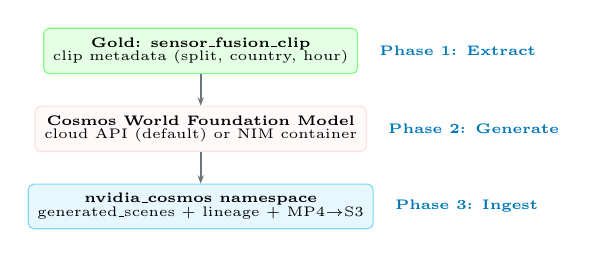
\begin{tikzpicture}[
    node distance=0.4cm,
    every node/.style={font=\tiny, align=center},
    box/.style={draw, rounded corners=2pt, minimum width=3.2cm,
                minimum height=0.55cm, fill=#1!10, draw=#1!50},
    box/.default=accent,
    arr/.style={-{Stealth[length=3pt]}, thick, muted},
    phase/.style={font=\fontsize{4.5}{5.5}\selectfont\bfseries, accent},
  ]
  \node[box=green]  (gold) {\textbf{Gold: sensor\_fusion\_clip}\\[-1pt]{\fontsize{4.5}{5.5}\selectfont clip metadata (split, country, hour)}};
  \node[phase, right=0.15cm of gold] {Phase 1: Extract};

  \node[box=pink, below=0.4cm of gold] (cos) {\textbf{Cosmos World Foundation Model}\\[-1pt]{\fontsize{4.5}{5.5}\selectfont cloud API (default) or NIM container}};
  \node[phase, right=0.15cm of cos] {Phase 2: Generate};

  \node[box=cyan, below=0.4cm of cos] (out) {\textbf{nvidia\_cosmos namespace}\\[-1pt]{\fontsize{4.5}{5.5}\selectfont generated\_scenes + lineage + MP4$\to$S3}};
  \node[phase, right=0.15cm of out] {Phase 3: Ingest};

  \draw[arr] (gold) -- (cos);
  \draw[arr] (cos)  -- (out);
\end{tikzpicture}

\vspace{6pt}
\raggedright
{\footnotesize\textbf{\textcolor{accent}{DESIGN DECISIONS}}}\\[3pt]
{\scriptsize
\begin{itemize}\setlength\itemsep{2pt}
  \item \textbf{Separate namespace} (\texttt{nvidia\_cosmos}) --- droppable without affecting base lakehouse
  \item \textbf{Read-only on Gold} --- never writes to nvidia\_bronze/silver/gold
  \item \textbf{Dual backend} --- cloud API avoids GPU requirement during dev;
        NIM container for dedicated hardware
  \item \textbf{Config-driven variations} --- new weather/lighting conditions via dict entry, no code changes
\end{itemize}
}

\end{column}

\begin{column}{0.43\textwidth}

{\footnotesize\textbf{\textcolor{accent}{VARIATIONS (6 DEFAULT, EXTENSIBLE)}}}\\[3pt]
{\scriptsize
\fcolorbox{muted!30}{muted!5}{\strut Fog}\;
\fcolorbox{blue!30}{blue!5}{\strut Rain}\;
\fcolorbox{violet!30}{violet!5}{\strut Night}\;
\fcolorbox{gray!40}{gray!10}{\strut Snow}\;
\fcolorbox{gold!40}{gold!8}{\strut Golden hour}\;
\fcolorbox{muted!30}{muted!5}{\strut Overcast}
}

\vspace{6pt}
{\footnotesize\textbf{\textcolor{accent}{END-TO-END TEST RESULTS}}}\\[2pt]
{\scriptsize
\begin{tabular}{@{}lr@{}}
\toprule
Metric & Result \\
\midrule
Clips processed & \textbf{\textcolor{gold}{3}} \\
Variations per clip & \textbf{\textcolor{gold}{3}} \\
Videos generated & \textbf{\textcolor{gold}{9}} \\
Metadata rows (Iceberg) & \textbf{\textcolor{gold}{9}} \\
Lineage rows (Iceberg) & \textbf{\textcolor{gold}{9}} \\
Trino queryable & \textbf{\textcolor{good}{Yes}} \\
\bottomrule
\end{tabular}
}

\vspace{6pt}
{\footnotesize\textbf{\textcolor{accent}{STATUS}}}\\[3pt]
{\scriptsize
\begin{itemize}\setlength\itemsep{1pt}
  \item[\textcolor{good}{\checkmark}] Pipeline code complete (5 modules)
  \item[\textcolor{good}{\checkmark}] End-to-end tested with mock server
  \item[\textcolor{good}{\checkmark}] Dual backend (cloud API + NIM)
  \item[\textcolor{gold}{$\circ$}] Validate with live NVIDIA API
  \item[\textcolor{gold}{$\circ$}] Run at scale on full Gold dataset
\end{itemize}
}

\vspace{6pt}
{\footnotesize\textbf{\textcolor{accent}{PRODUCTION PROJECTION}}}\\[2pt]
{\scriptsize
\textbf{\textcolor{gold}{311\,K}} clips $\times$
\textbf{\textcolor{gold}{6}} variations =
\textbf{\textcolor{gold}{$\sim$1.87\,M}} videos\\
{\tiny\color{muted} Embarrassingly parallel --- scales linearly with API throughput or NIM replicas.}
}

\end{column}
\end{columns}

\end{frame}

\end{document}
